\documentclass{article}
\usepackage[utf8]{inputenc}
\usepackage{graphicx}
\graphicspath{ {./Imagenes/} }
\usepackage{multicol}
\usepackage[spanish, english]{babel}
\usepackage[left=3cm,right=3cm,top=3cm,bottom=3cm]{geometry}

\providecommand{\keywords}[1]{
  \small	
  \textbf{\textit{\quad \quad Keywords: }} #1}

\providecommand{\pclave}[1]{
  \small	
  \textbf{\textit{\quad \quad Palabras Clave: }} #1}

%Idiomas: \selectlanguage{english} \selectlanguage{spanish}

\begin{document}

\title{Trabajo Encargado N°1: Comparativa Frameworks de pruebas}

\begin{titlepage}
\begin{figure}[htb]
\begin{center}

\includegraphics[width=5cm]{logo.png}
\end{center}
\end{figure}
\vspace*{-0.25in}
\begin{center}
\large{UNIVERSIDAD PRIVADA DE TACNA}\\
\vspace*{-0.025in}
INGENIERIA DE SISTEMAS  \\

\vspace*{0.5in}
\begin{large}
TITULO:\\
\end{large}

\vspace*{0.1in}
\begin{Large}
\textbf{Comparativa de Frameworks de Pruebas} \\
\end{Large}

\vspace*{0.3in}
\begin{Large}
\textbf{CURSO:} \\
\end{Large}

\vspace*{0.1in}
\begin{large}
CALIDAD Y PRUEBAS DE SOFTWARE\\
\end{large}

\vspace*{0.3in}
\begin{Large}
\textbf{DOCENTE:} \\
\end{Large}

\vspace*{0.1in}
\begin{large}
 Ing. Patrick Cuadros Quiroga\\
\end{large}

\vspace*{0.2in}
\vspace*{0.1in}
\begin{large}

Integrantes: \\
\begin{flushleft}
Sivirichi Falcón, Ricardo Alonso\hfill(2018060905) \\
Chambilla Maquera, Araceli Noemi\hfill(2018060897)\\
Arenas Paz Soldan, Miguel Jesus\hfill(2017059282)\\
Cotrado Marino, Ana Luz\hfill(2018060907)\\

\end{flushleft}
\end{large}

\vspace*{0.1in}
\begin{large}
Tacna - Perú\\
2020
\end{large}
\end{center}
\end{titlepage}

\selectlanguage{spanish}
\begin{abstract}
\quad En este articulo de investigación expondremos sobre los frameworks de pruebas de
apis asi como también se hablara sobre lo que es
una api y como funciona también compararemos
dos frameworks de pruebas de apis.

\end{abstract}
\pclave{Frameworks de pruebas.}

\selectlanguage{english}
\begin{abstract}
\quad In this research article we will discuss about the testing frameworks of
apis as well as they will also talk about what it is
an api and how it works we will also compare
two apis testing frameworks.

\end{abstract}
\keywords{Test Framework.}

\begin{center}\rule{1\textwidth}{0.05mm} \end{center}

\selectlanguage{spanish}

\begin{multicols}{2}
\section{Introducción}
Para producir software con un nivel de calidad insuciente puede ser un pésimo negocio.
Según Stadish Group  en  su  informe de  2015(Chaos Report)[1],  el  52Solo   ],  el  52Solo   el  29\%, llegan   a  el  éxito,   No solo  es suficiente con  que  una  aplicación funcione completamente , acorde a  su  propósito  , sino  que también debe satisfacer otros aspectos en términos de  seguridad , rendimiento, accesibilidad ,etc.   Por eso   el  objetivo  de  cualquier   organización  que  se dedique a  la  industria  del  software debe  producir software de  calidad  .  
La calidad  debe ser  una  exigencia  obligada y cada
vez  son  mas  las  empresas que  consideran el 
aseguramiento de la calidad. Una  de  las partes
importantes que  componen las tareas propias de un 
sistema de  aseguramiento de la calidad  que  son  las
pruebas de  software.   Existen  pruebas unitarias,
de  integración, funcionales, de  rendimiento, etc. 
En la actualidad existen herramientas que permiten generar 
y ejecutar scripts, pequeños  programas que  permiten 
interactuar con una aplicación dada, simulando las acciones 
que podría realizar un usuario real, estas herramientas
ayudan a incrementar la productividad como  frameworks 
de pruebas para Apis.

\section{Desarrollo}
\subsection{¿Que es un API?}
API (Application Programen Interface) Es una interfaz informática con la cual se puede intercambiar y comunicar datos entre dos sistemas de software separado. API incluye varias funciones/subrutinas que puede realizar otro sistema de software. La API define las solicitudes que se pueden realizar, como realizar las solicitudes, los formatos de datos que se pueden utilizar, etc. entre dos sistemas de software.

\subsection{API Rest}

\subsection{¿Que son las pruebas de API?}
PRUEBA DE API es un tipo de prueba de software que valida las interfaces de programación de aplicaciones (API). El proposito de las pruebas de API es verificar la funcionalidad, confiabilidad, rendimiento y seguridad de las interfaces de programación. En API Testing, en lugar de utilizar entradas y salidas de usuario estándar (teclado), utiliza software para enviar llamadas a la API, obtener resultados y anotar la respuesta del sistema. Las pruebas de API son muy diferentes de las pruebas de GUI y no se concentran en la apariencia de una aplicacion. Se concentra principalmente en la capa de logica empresarial de la arquitectura de software.

\subsection{Frameworks de Pruebas de APIs}
\subsubsection{Postman}

Herramienta que se utiliza, sobre todo, para el testing de API REST, aunque también admite otras funcionalidades que se salen de lo que engloba el testing de este tipo de sistemas.
\begin{center}
    
\includegraphics[width=5cm]{Imagenes/postman.png}
\end{center}
Gracias a esta herramienta, además de testear,consumir y depurar API REST, podremos monitorizarlas, escribir pruebas automatizadas para ellas,documentarlas, simularlas, etc.

Quizás sea una de las herramientas mas utilizadas para hacer testing exploratorio de este tipo de sistemas. Puede que no sea la mejor forma de escribir pruebas automatizada, pero sin duda es una de las mas favorables para equipos con poca experiencia en programación, y sobre todo para hacer testing de todo tipo en general de API REST.

\textbf{Características}
\begin{itemize}
\item Crear Peticiones, te permite crear y enviar peticiones http a servicios REST mediante un interface
gráfico. Estas peticiones pueden ser guardadas y reproducidas a posterior.
\item Definir Colecciones, mediante Postman podemos
agrupar las APIs en colecciones. En estas colecciones podemos definir el modelo de autentificacion
de las APIs para que se añada en cada petición. De 
igual manera podemos ejecutar un conjunto de test,
ası como definir variables para la colección. 
\item Gestionar la Documentación, genera documentación basada en las API y colecciones que 
hemos creado en la herramienta. Además esta documentación podemos hacerla publica.
\item Entorno Colaborativo, permite compartir las API
para un equipo entre varias personas. Para ello se apoya en una herramienta de colaborativa en Cloud.
\item Genera código de invocación, dado un API es capaz de generar el código de invocación para diferentes lenguajes de programacion: C, cURL, C#, Go,Java, JavaScript, NodeJS, ObjectiveC, PHP, Python, Ruby, Shell, Swift,etc.
\item Establecer variables, con Postman podemos crear variables locales y globales que posteriormente utilicemos dentro de nuestras invocaciones o pruebas.
\item Soporta Ciclo Vida API management, desde Postman podemos gestionar el ciclo de vida del API Management, desde la conceptualizacion del API, la definición del API, el desarrollo del API y la monitorización y mantenimiento del API. 
\item Crear mockups, mediante Postman podemos crear un servidor de mockups o sandbox para que se puedan testear nuestras API antes de que estas estén desarrolladas
\end{itemize}

\textbf{Ventajas}

\begin{itemize}
 \item Permite la colaboración entre miembros del equipo.
 \item Tiene una interfaz mas intuitiva y atractiva. 
 \item Posee extensión para Google Chrome, por lo 
tanto no es necesario instalar la aplicación de 
escritorio.
 \item Como ya mencionamos en la descripción, tiene 
una opción muy interesante, que son las coleccines, que funciona básicamente como una
base de datos de peticiones.
 \item Es extensible y se puede integrar con otras herramientas, por ejemplo ejecutando las suites de
prueba desde un motor de CI/CD.
 \item Permite agregar scripts en lenguaje Javascript
para agregar validaciones, configurar y/o automatizar pruebas (esto se realiza directamente
en la petición).
\end{itemize}

\subsubsection{SoapUI}
SoapUI es una herramienta desarrollada en Java, utilizada para pruebas de aplicaciones con arquitectura SOA o REST. Soporta múltiples protocolos como SOAP, REST, HTTP, JMS y JDBC.
\begin{center}
    
\includegraphics[width=5cm]{Imagenes/soapui.png}
\end{center}

La herramienta cuenta con una versión de código abierto y otra versión paga desarrollada por la compañía SmartBear. La herramienta SoapUI se creo inicialmente para probar los servicios SOAP. Luego, se extendió a los servicios web RESTful.
Para un usuario nuevo puede requerir una mediana curva de aprendizaje ya que la misma en ocasiones no resulta tan intuitiva.

\textbf{Características}

La herramienta ofrece muchas características avanzadas para las pruebas API, incluyendo:
\begin{itemize}
    \item Genera pruebas fácilmente usando arrastrar y soltar, apuntar y hacer clic.
    \item Potentes pruebas basadas en datos con datos de archivos y bases de datos.
    \item Los scripts se pueden reutilizar fácilmente.
    \item Servicios de mocks con mocking RESTful.
    \item Pruebas asíncronas.
\end{itemize}

\textbf{Ventajas}

\begin{itemize}
    \item Tiene una mejor integración que Postman para trabajar con el protocolo SOAP (ya que inicialmente estaba pensada para eso).
    \item Es un proyecto mas maduro y tiene más tiempo en el mercado.
    \item Es una aplicación más orientada a testing y no simplemente a consumir una API, documentarla y publicarla. Permite estructurar las pruebas en test suites, test cases y test steps.
    \item La ejecución de pruebas se puede integrar con herramientas tales como: Maven, motores de CI/CD, etc.
    \item Permite agregar scripts en lenguaje Groovy.Esto permite agregar validaciones, configurar y/o automatizar pruebas.
\end{itemize}

\section{Comparativa Postman y SoapUI}

\begin{itemize}
    \item Generación automatizada de aserciones: esta capacidad implica analizar API y generar aserciones automáticamente. Se espera que ahorre tiempo al generar aserciones manualmente para las API. Las dos herramientas proporcionan funciones básicas para generar scripts de aserción basados en algunas plantillas o reglas predefinidas.
    \item Informes de prueba: las dos herramientas proporcionan capacidades para reportar resultados de prueba de API. Postman genera informes en formatos JSON y HTML. Para SoapUI, la capacidad de producir informes de prueba detallados se encuentra en la edición comercial.
    \item Lenguajes de scripting: todas las herramientas admiten lenguajes basados en Java.
    \item Pruebas de UI web y aplicaciones móviles: en el desarrollo de una aplicación multiplataforma, el equipo realiza pruebas de aplicaciones móviles y UI web además de las API de pruebas. Por lo tanto, existe un déficit entre Postman y SoapUI, ya que no permiten a los desarrolladores y tester usar la misma herramienta, compartir y colaborar en los mismos casos de prueba.
\end{itemize}

\end{multicols}

\begin{center}
    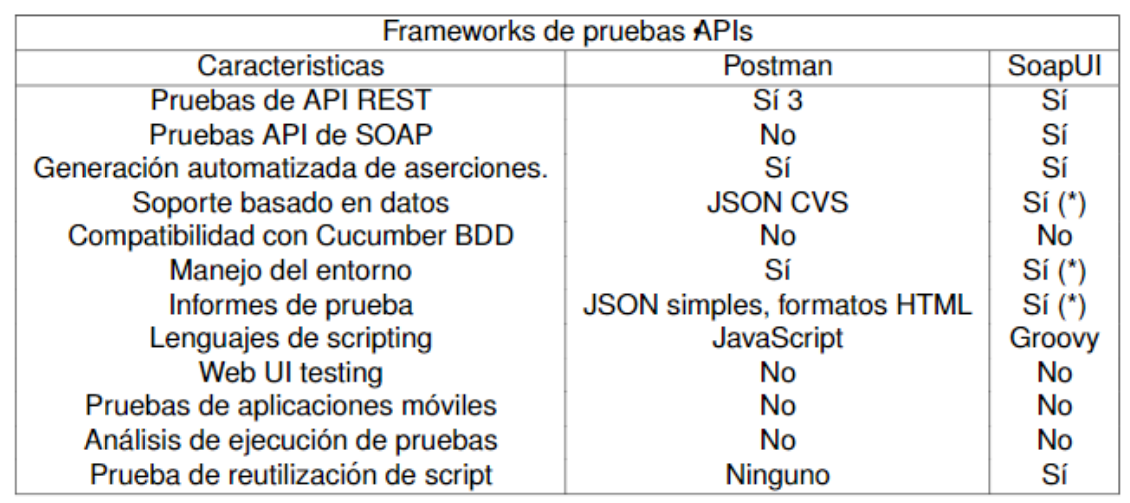
\includegraphics[width=12cm]{Imagenes/comparativa.png}
\end{center}

\begin{multicols}{2}
\section{Conclusión}
Las pruebas en un proyecto de APIs son fundamentales, nos garantizan que podemos hacer cambios de versiones, actualizaciones, corrección de bugs o nuevas implementaciones garantizando que la especificación coincide con el método y que
cualquier cliente que va a consumir nuestras APIs lo puede hacer sin ningún problema.

\section{Recomendaciones}
\subsection{Planificación previa}
Desde el inicio de la estimación de casos de
prueba, es aconsejable asignar prioridades de ejecución: Alta, Media, Baja y palabras clave como
Regresión, Sanidad, etcétera para los casos de
prueba. De esta manera se puede hacer un filtrado
rápido por prioridades y etiquetas, que permitan
diferenciar rápidamente cuáles deberían ser los
casos más importantes.
\subsection{Uso de técnicas de diseño de casos de prueba}
Entidades como International Software Testing
Qualifications Boardy American Society for Quality
mencionan varias técnicas para la creación de casos
de prueba que permiten una mejora,de tal manera
que al aplicarlas se obtienen menos casos de
prueba y un mayor factor de cobertura o bien una
base de creación empírica.
Al tener un menor número de casos de prueba,
se reducen las pruebas exhaustivas y tiempos de
ejecución.
\subsection{Clasificación de suites}
La división de casos de prueba según los módulos
de un sistema, facilitará la selección de casos al momento
de construir un Plan de Pruebas para Regresión.
En las carpetas o suites deberían evitarse nombres
ambiguos o diferentes a lo definido en el requerimiento,
o en los nombres que se muestran en
el sistema.
Si la herramienta de manejo de casos de prueba
lo permite, lo ideal es organizar las suites mediante
jerarquías según la misma aplicación para que
la selección de casos de prueba por componente
pueda ser natural. Por ejemplo, si el módulo transferencias”
tiene como opciones ”Transferencias locales”,
”Transferencias a terceros”, ”Transferencias
internacionales”, debería existir un folder padre llamado
”TRANSFERENCIAS”, con 3 carpetas hijas,
de manera tal que la carpeta llamada ”Transferencias”
tenga como opciones ”Transferencias locales”,
”Transferencias a terceros”, ”Transferencias internacionales”.
Este tipo de organización es útil para mantener los
casos de prueba ordenados y agilizar la búsqueda
de casos de prueba. Sin embargo, no se debe
abusar de la jerarquía, pues llegar a tener más de
4 ó 5 niveles de profundidad se torna poco eficiente.
\subsection{Programación de mantenimientos}
Conforme nuestra aplicación crece o sufre cambios
y mejoras, se hace más necesario dedicar
tiempo a revisar si estos cambios afectan nuestros
casos actuales, invalidándolos o requiriendo actualización. Si sabemos que el cambio los afectará, se
deberían incluir tareas de actualización.
Si estamos bajo un modelo de un sistema antiguo
con casos que nunca han tenido mantenimiento, se
recomienda incluir tareas periódicas para la revisión
de todos los casos existentes.
\subsection{Definición del tipo de Regresión a realizar}
No todas las pruebas de regresión implican una
ejecución del 100
En estos casos es necesario un análisis de dependencias
para tener certeza de que los cambios
por aplicar efectivamente no afectan otras partes
\subsection{Automatización}
Las pruebas de regresión suelen ser procesos largos
y al incorporar pruebas de automatización se
consiguen varias ventajas.
Primeramente, la capacidad de ejecución aumenta,
al tiempo que la duración de las pruebas se
reduce.
Los scripts pueden ejecutarse tantas veces como
se requiera sin que esto implique desgaste en el
equipo.
Asimismo, se pueden incorporar diferentes ambientes
en la prueba sin que esto aumente el tiempo
de las mismas, pues pueden ejecutarse en paralelo.
\end{multicols}

\begin{thebibliography}{XXX0000}
    \bibitem{FRE2008} Freeman, E., Robson, E., Bates, B., y Sierra, K. (2008). Head first design patterns. "O' Reilly Media, Inc.".

    \bibitem{DOC2017} Dockins, K. (2017). Design Patterns in PHP and Laravel. Apress. \\https://allitbooks.net/web-development/2056-design-patterns-php-laravel.html
    
    \bibitem{FRE2008} 
    FEDERICO TOLEDO,(2020),API testing con Postman y SoapUI.
    https://www.federico-toledo.com/api-testing-con-postman-y-soapui/
   
    \bibitem{COO2000} 
    SHANE HASTIE,S.H., & STEPHANE WOJEW-ODA, S. W. ,(2015),Standish 
    Group 2015 Chaos Report   Q&A with Jennifer Lynch. 
    InfoQ.https://www.infoq.com/articles/
  
    \bibitem{HUN2013}
    MICROSOFT.(S.  F.).CODIGOS DE ERROR DE LA API REST,MicrosoftDocs.  
    Recuperado el 2 de diciembre de 2020,de:https://docs. microsoft.com/es-es/partner/develop/
    \end{thebibliography}

\end{document}